\section{Statistical learning framework}

Let's start with the basic formal framework describing statistical learning theory. 


\subsection*{Papaya example}
We will start with an introductory example concerned with papayas. The task in our example is the following: 

\begin{itemize}
  \item \begin{tikzborder}{Boolean classification problem} We want to predict whether a tropical fruit (here a papaya) is tasty or not.\end{tikzborder}
  \item The decision shall be based on observations that we can make from the outside.
  \item \begin{tikzborder}{Supervised learning setting} We get a sample of papayas to try, which we will use as our \textit{training set}.
  \end{tikzborder}
\end{itemize}

\begin{figure}[h]
  \centering
  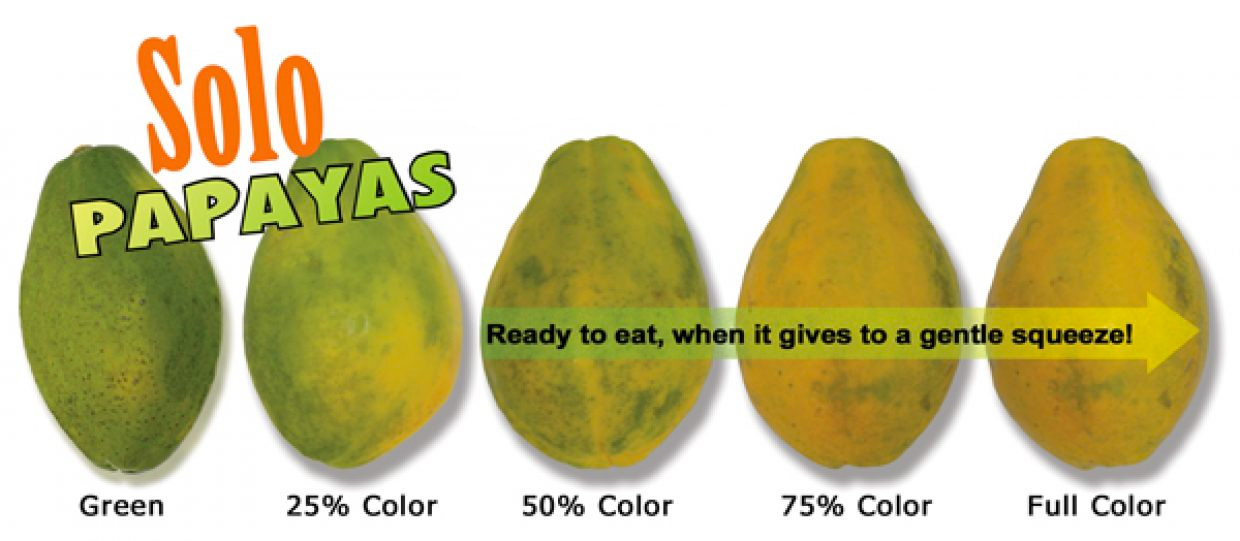
\includegraphics[width=0.6\textwidth]{assets/slf/papayas.jpg} 
  \caption{Papaya with different features}
\end{figure}

\begin{tikzborder}{Feature selection} As our first step, we need to select features.\end{tikzborder} Based for example on previous experience with other fruits, we decide to base our decision on these two features of papayas:
\begin{itemize}
  \item Colour, ranging from green through yellow and red to brown
  \item Softness, ranging from hard to mushy
\end{itemize}

When we fill a diagram with our training data to visualize the features and the correct labels.

\begin{figure}[h]
  \centering
  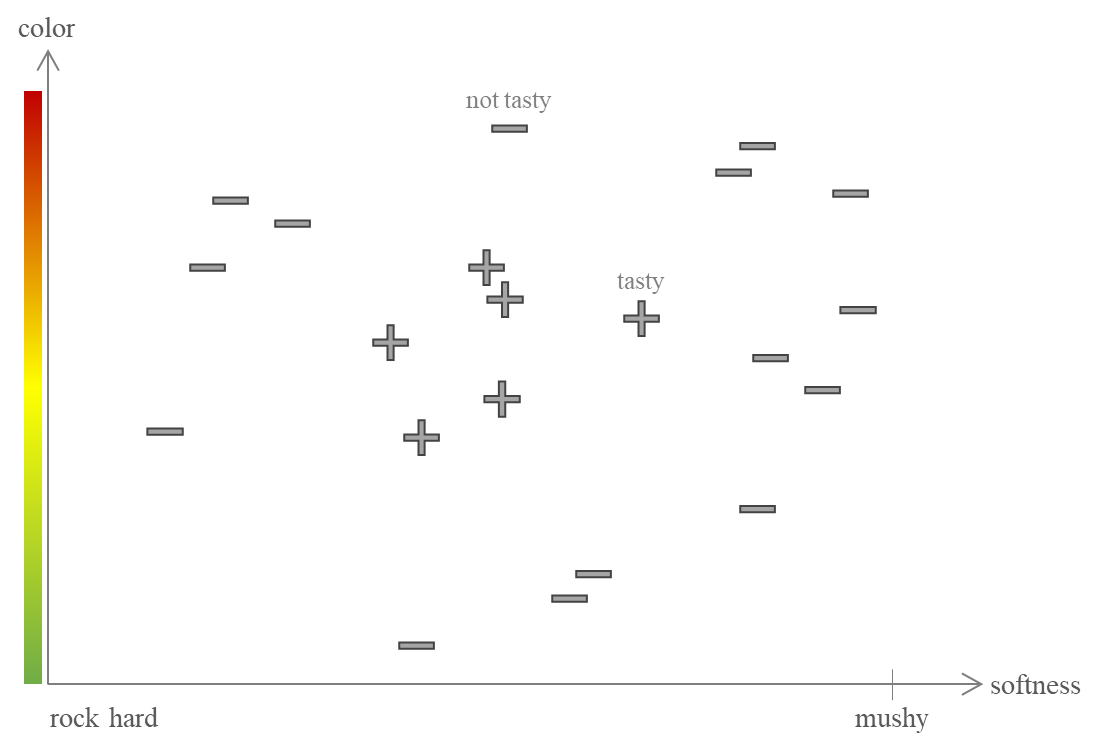
\includegraphics[width=0.7\textwidth]{assets/slf/papaya_testdata__0.png} 
  \caption{Papaya features}
\end{figure}

Next, we select a model and try to fit it optimally with our training data. For that, parameter fitting is applied.
Consider for example a simple \begin{tikzborder}{parametric model}{parametric model}\end{tikzborder} where the features have to lie in a certain range.
\begin{equation*}
  \begin{array}{@{}l@{}}
      \begin{minipage}[b]{0.4\textwidth}
          \begin{itemize}
              \item Color: $[c_{\min}, c_{\max}]$
              \item Softness: $[s_{\min}, s_{\max}]$
          \end{itemize}
      \end{minipage}
  \end{array}
  \left.\begin{array}{@{}c@{}}
      \\
      \\
      \\
  \end{array}\right\}\begin{minipage}{0.6\textwidth}
    4 parameters to be estimated\\
    goal: make resulting hypothesis explaining data best
\end{minipage}
\end{equation*}


\begin{figure}[h]
  \centering
  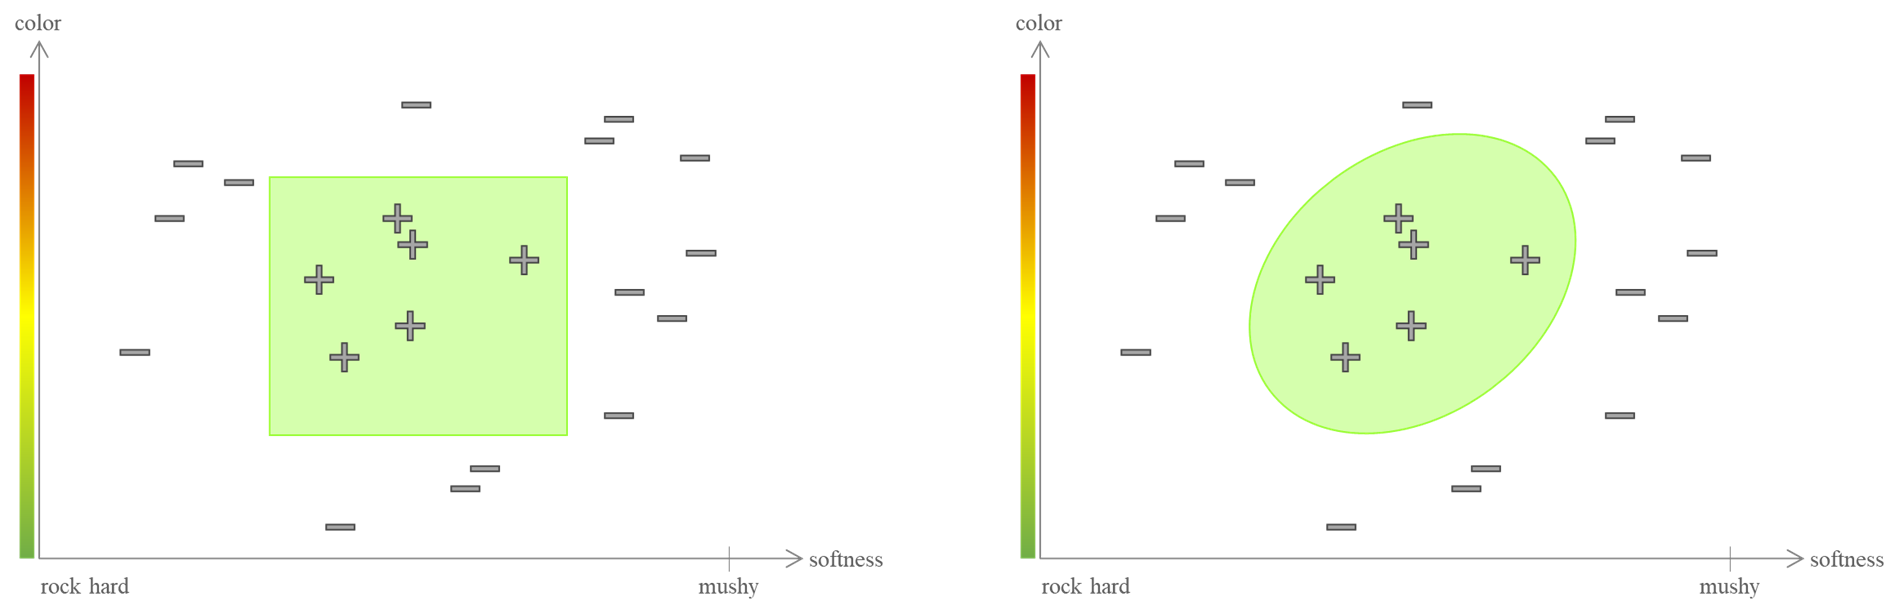
\includegraphics[width=0.9\textwidth]{assets/slf/papaya__1.png} 
  \caption{Papaya features}
\end{figure}